\newlength{\fh}\setlength{\fh}{95mm}%
\begin{fig}{\linewidth}
  \begin{minipage}[b]{.69\linewidth}\null
    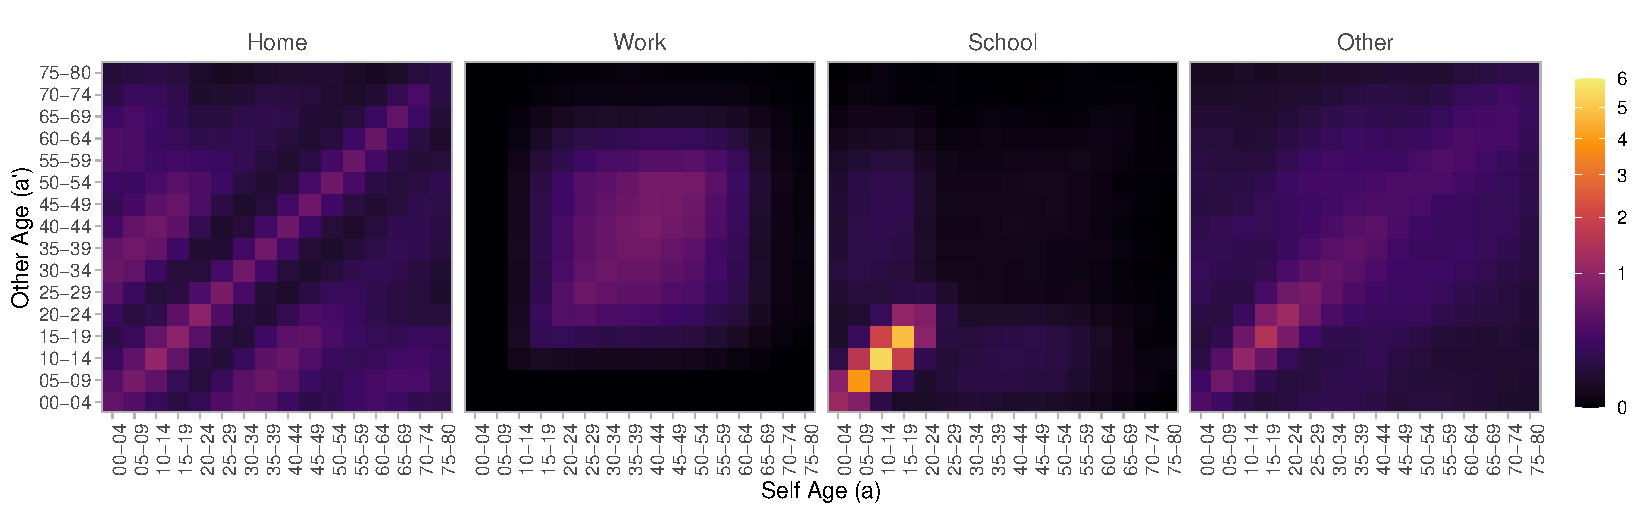
\includegraphics[height=\fh]{C4aa3}
    \vskip-\bigskipamount
    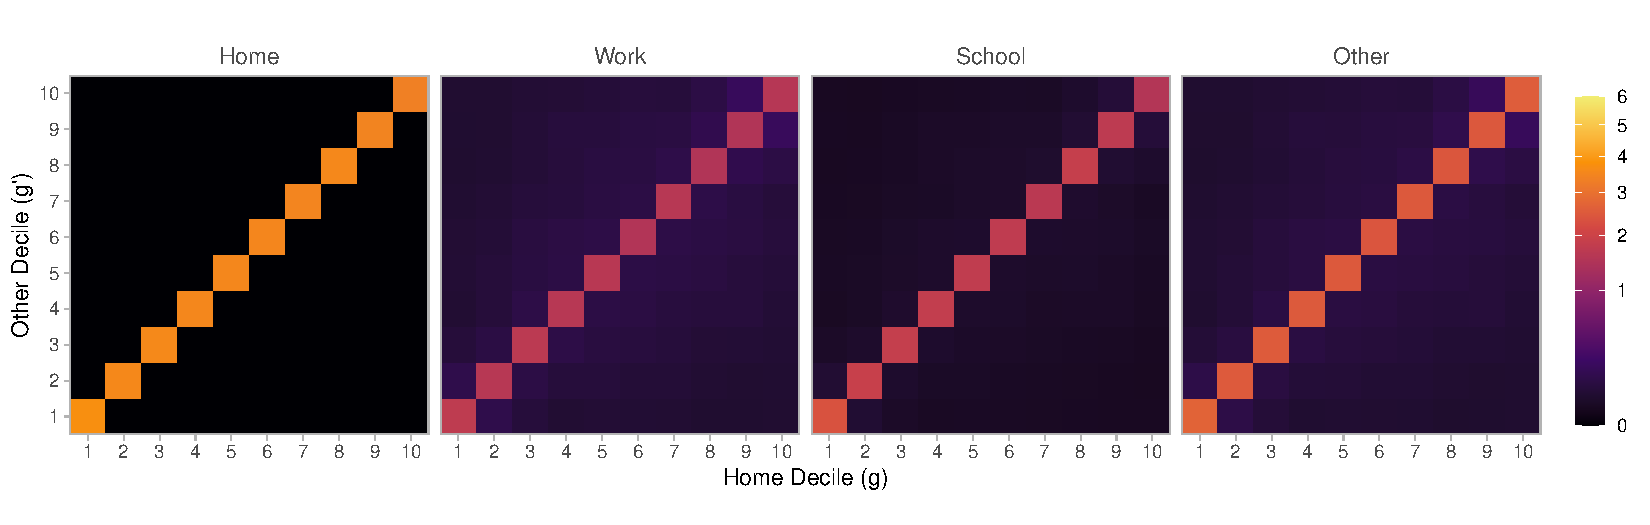
\includegraphics[height=\fh]{C4gg3}
  \end{minipage}%
  \begin{minipage}[b]{.31\linewidth}\null
    \begin{fig}{\linewidth}
      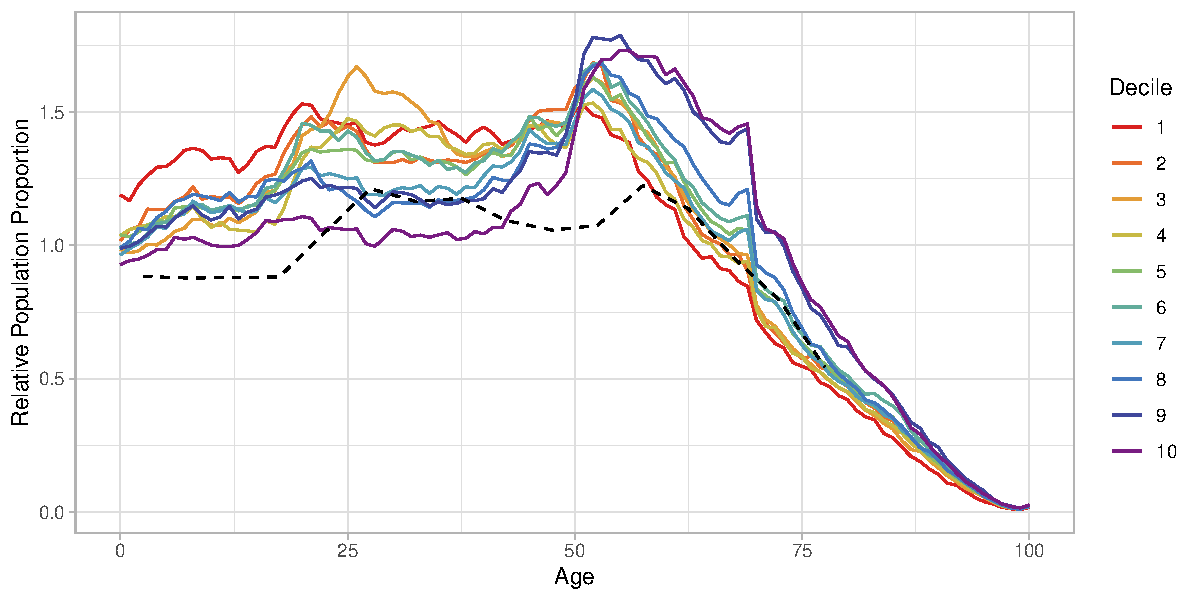
\includegraphics[width=\linewidth]{Pga}
      \caption{Relative age distribution by
        patch (colours \cite{StatsCan2016}) and
        overall (dotted \cite{Prem2021})}
      \label{fig:Pga}
    \end{fig}
    \bigskip\bigskip\bigskip\par
    \caption{Contact patterns: \# daily contacts per person, stratified by type,
      after relaxing all 3 assumptions.
      (a) Age patterns are similar to inputs from \cite{Prem2021}.
      (b) Patch patterns are dominated by within-patch contacts,
      due to both within-patch mobility and the home mixing pool model.
      Colour scale is square-root-transformed to improve perception.}
    \label{fig:panel-mix}\bigskip\bigskip
  \end{minipage}
\end{fig}
\begin{fig}{\linewidth}
  \begin{minipage}[b]{.69\linewidth}\null
    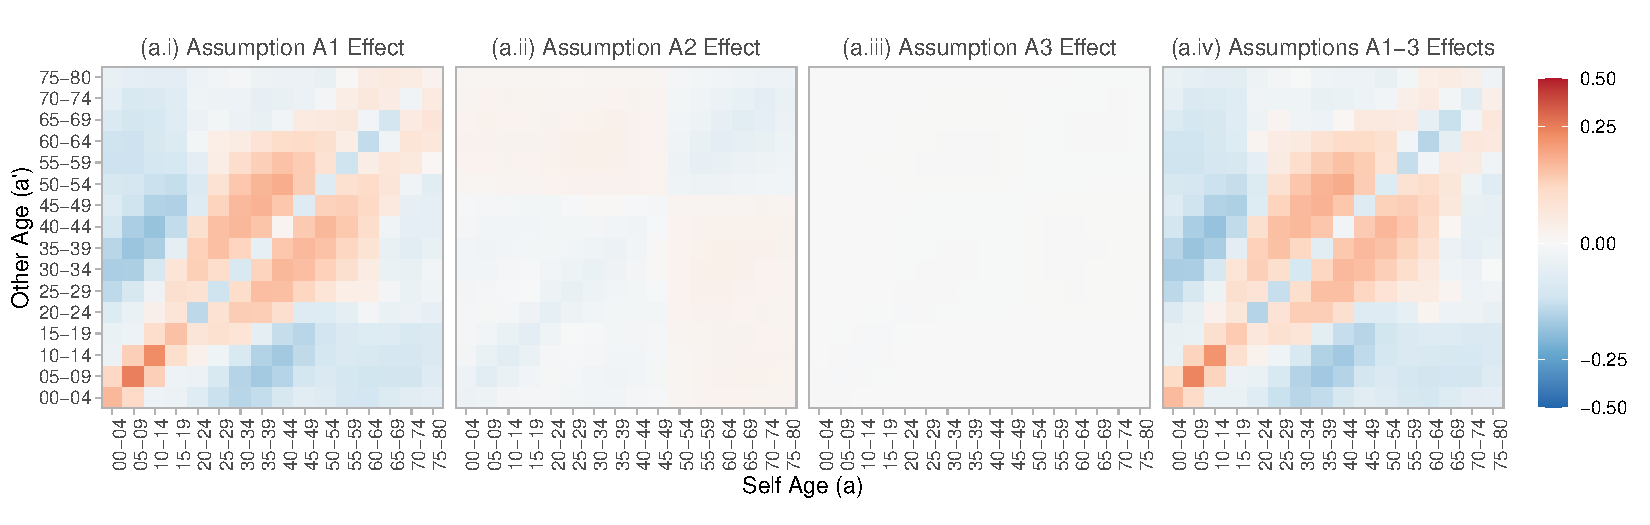
\includegraphics[height=\fh]{Daa-panel}
    \vskip-\bigskipamount
    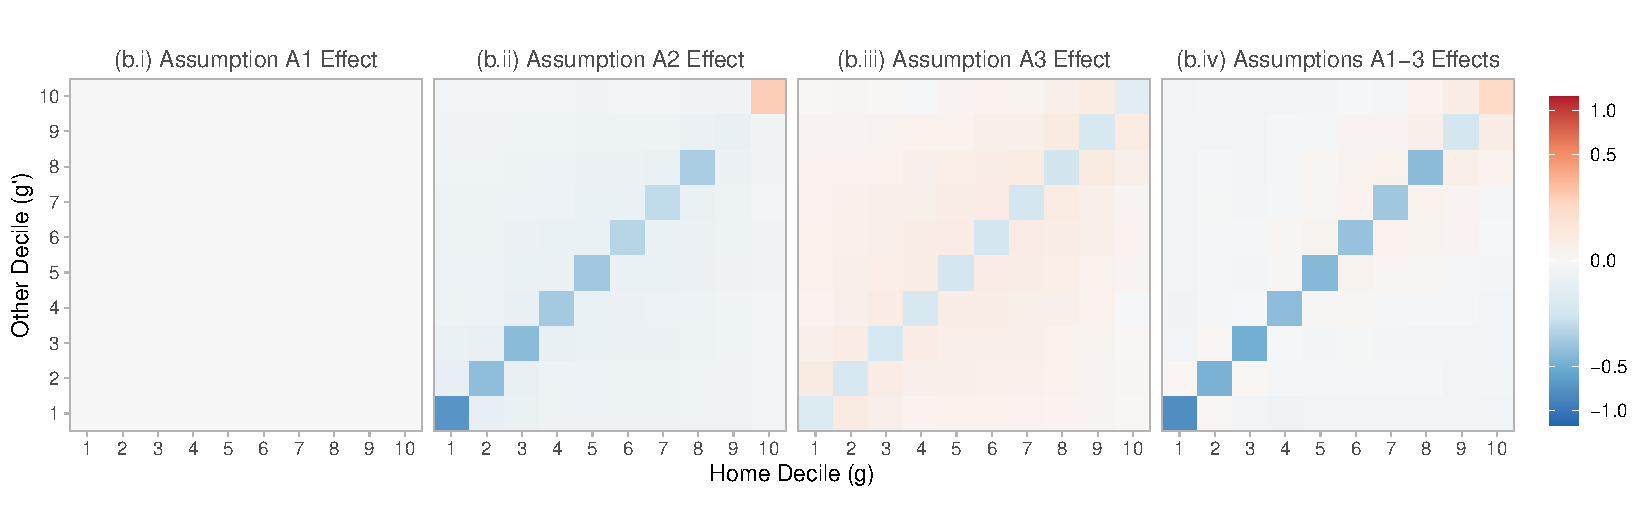
\includegraphics[height=\fh]{Dgg-panel}
  \end{minipage}%
  \begin{minipage}[b]{.31\linewidth}
    \caption{Differences in \# daily contacts per person (overall)
      estimated with vs (minus) without each assumption. Therefore:\\
      positive: \textcolor{Rd}{overestimation with assumption}\\
      negative: \textcolor{Bu}{underestimation with assumption}.\\
      Differences in (a) age patterns and (b) patch patterns.
      Individual effects of assumptions \ass1,~\ass2,~\ass3 in (i), (ii), and (iii);
      net effect of all three in (iv).
      Colour scale is square-root-transformed to improve perception.}
    \label{fig:panel-diff}\bigskip\bigskip
  \end{minipage}
\end{fig}\vskip-1ex